\begin{figure*}[t]
\centering
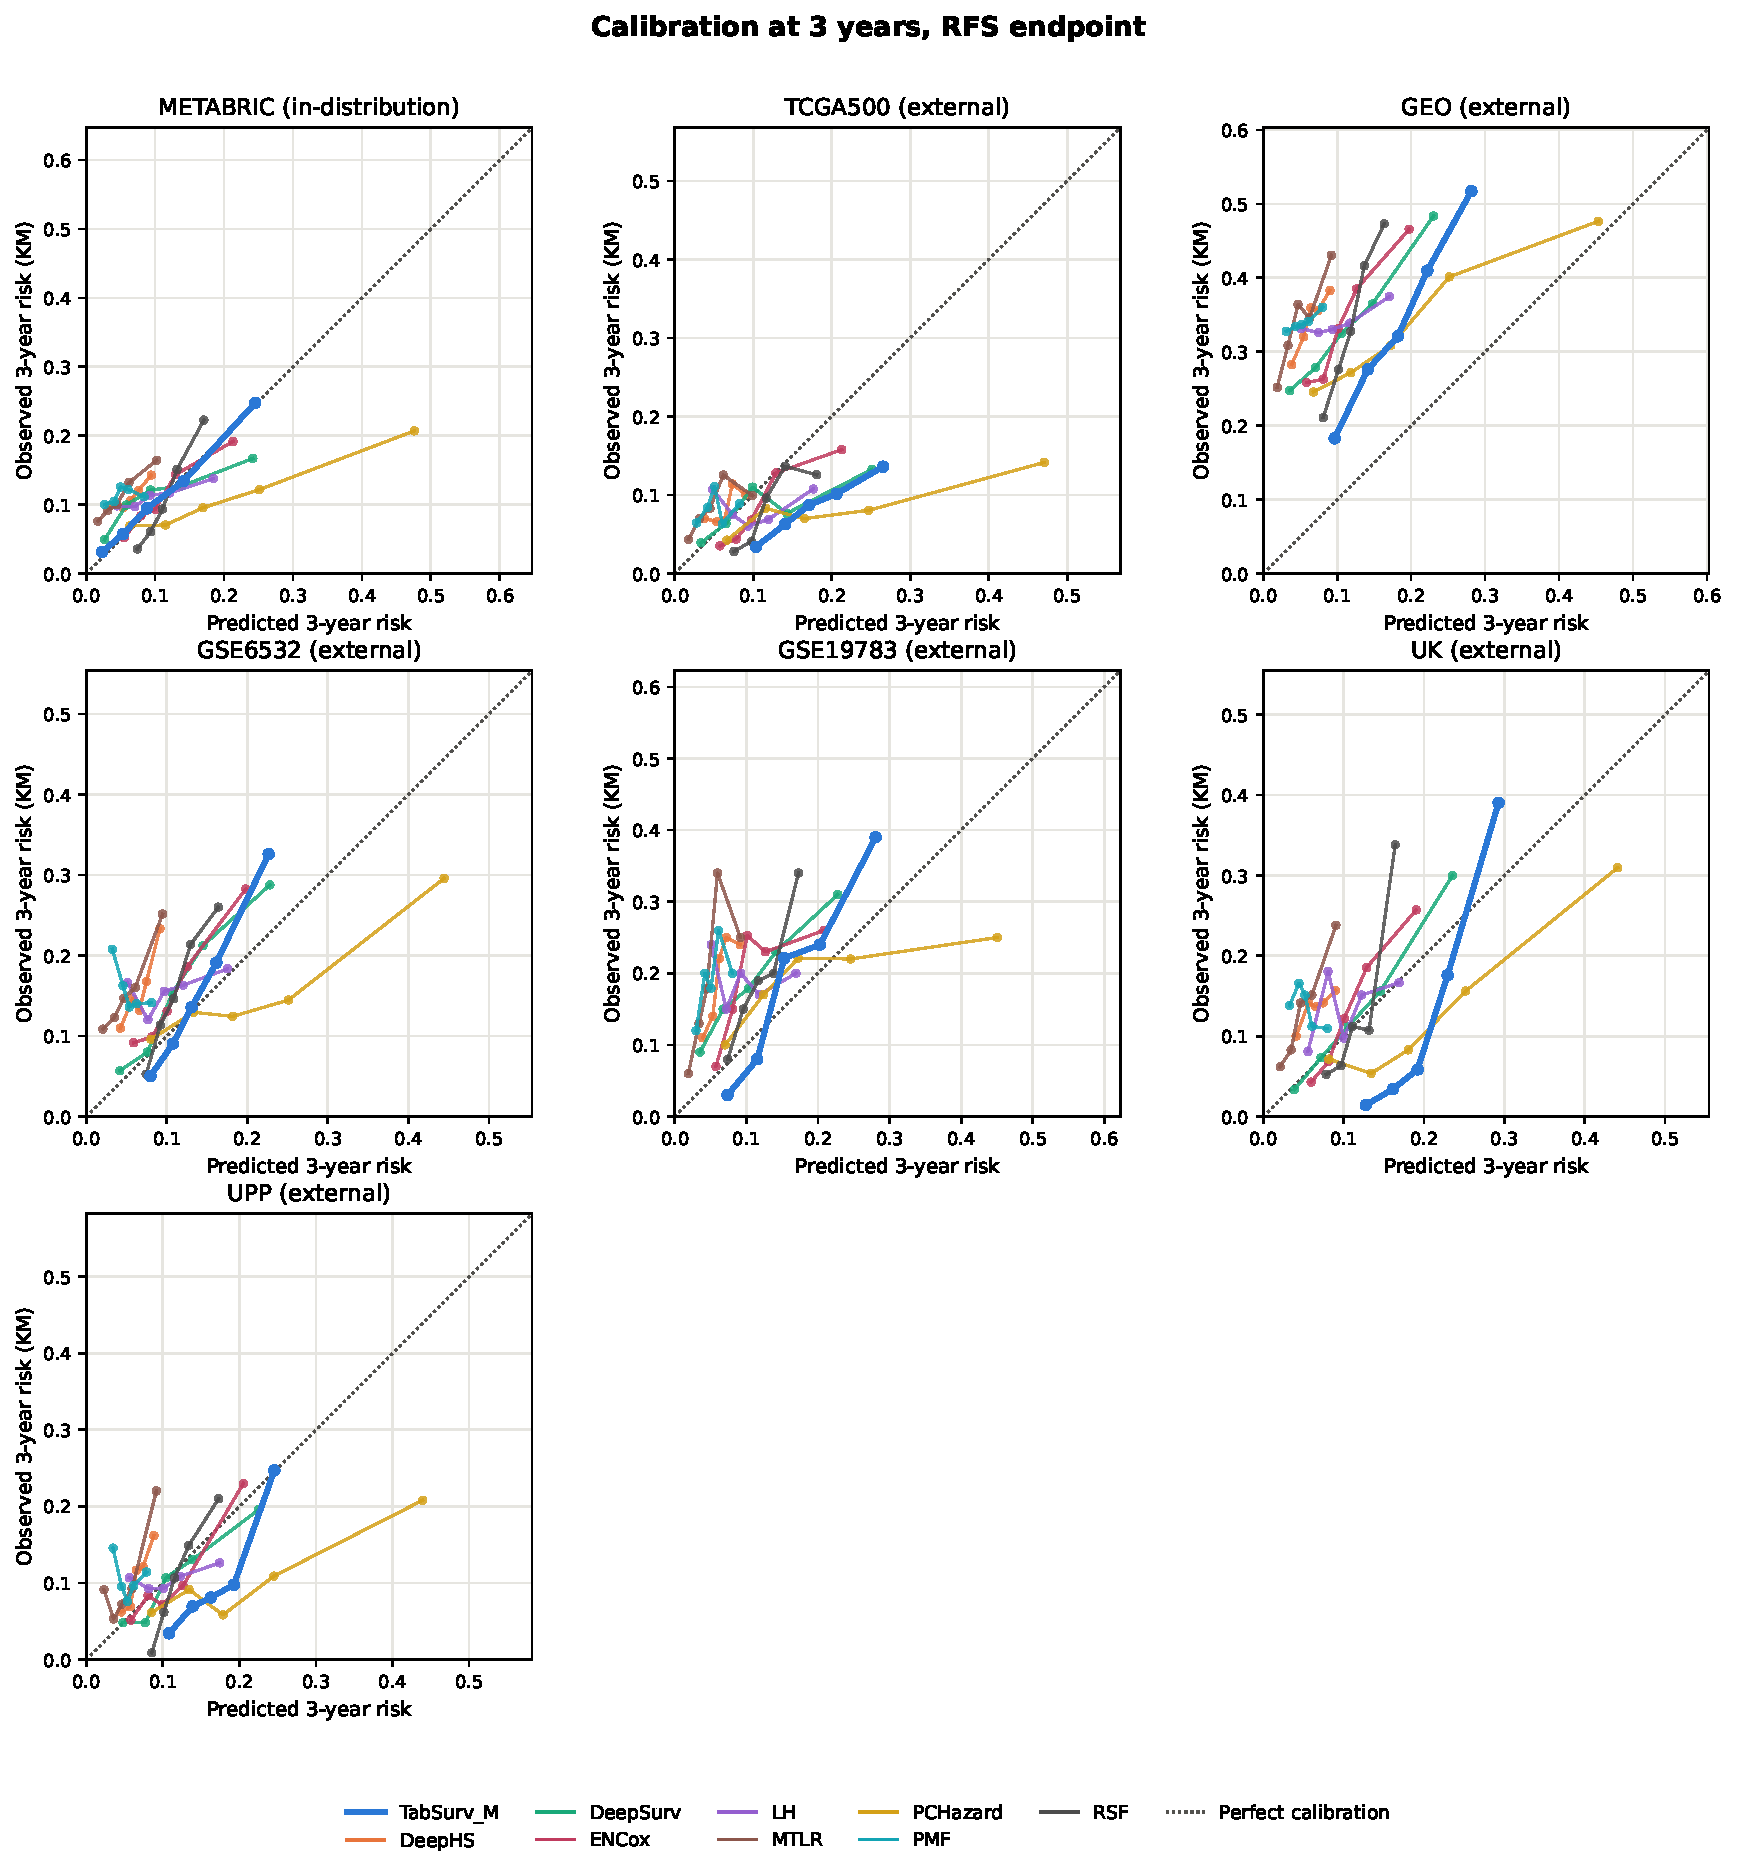
\includegraphics[width=\textwidth]{Fig_S_calibration_RFS_3y.pdf}
\caption{Calibration of predicted 3-year RFS risk in every cohort. Each point is a risk group: mean predicted risk of an event by 3 years against the Kaplan--Meier observed risk in that group, averaged over five seeds. The dotted diagonal marks perfect calibration. TabSurv\_M is shown as a thick blue line. Panels marked as having too short follow-up have no patients at risk beyond 3 years.}
\label{fig:supp_calibration_rfs_3y}
\end{figure*}

\begin{figure*}[t]
\centering
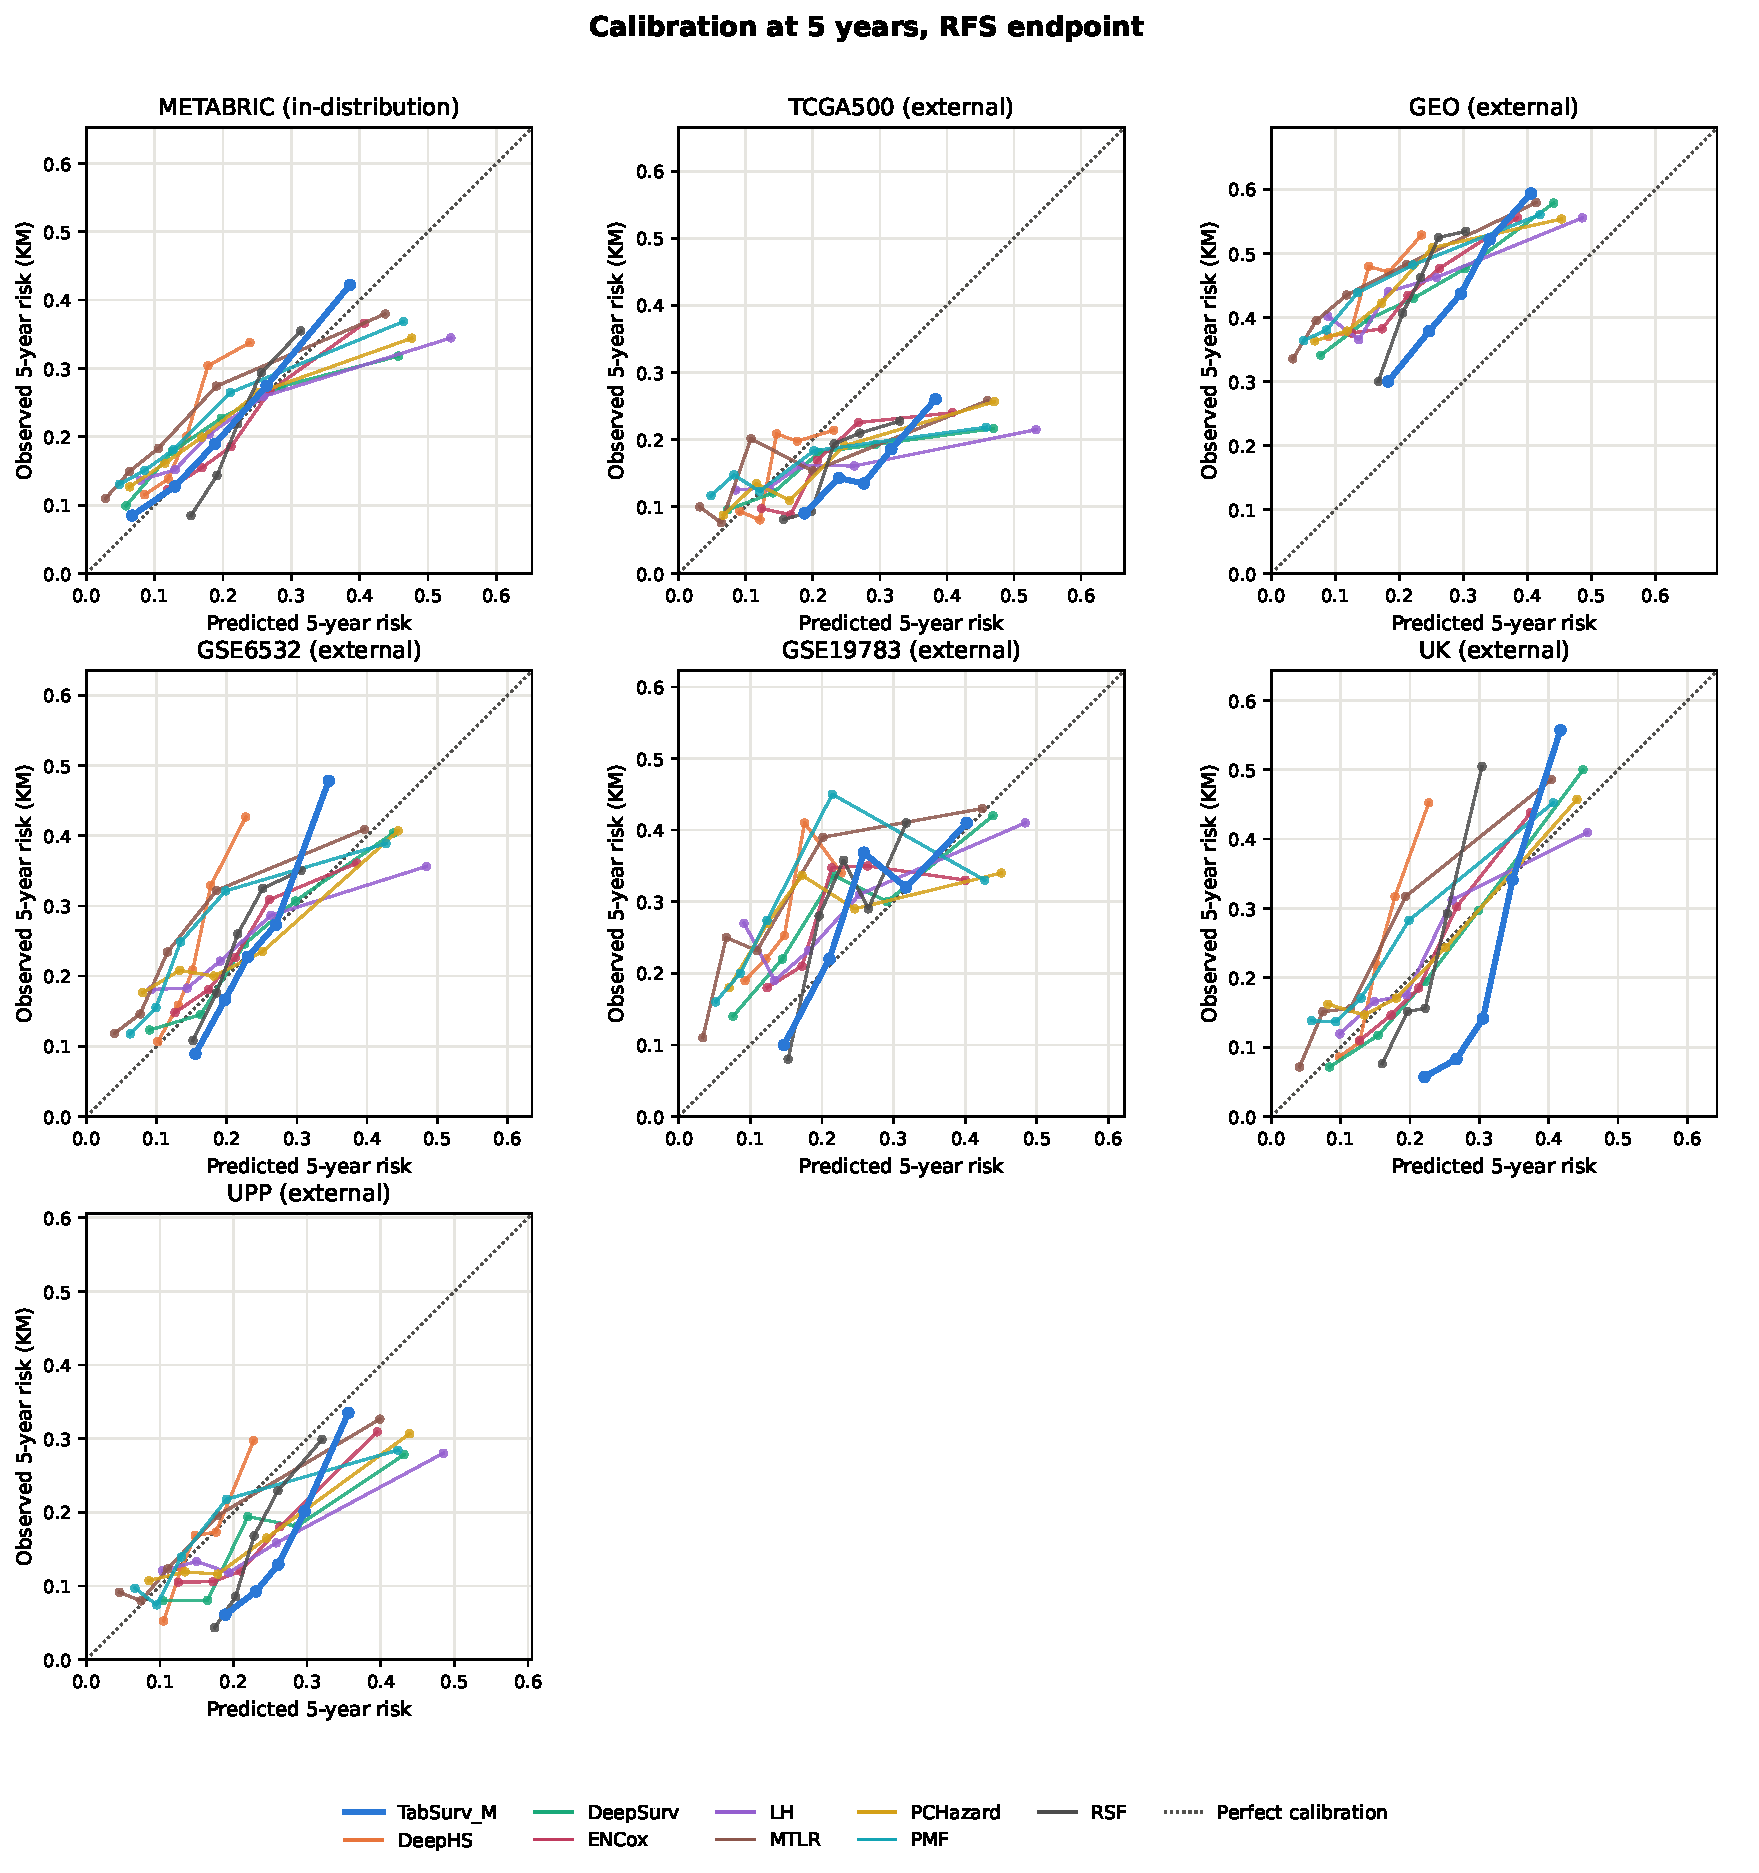
\includegraphics[width=\textwidth]{Fig_S_calibration_RFS_5y.pdf}
\caption{Calibration of predicted 5-year RFS risk in every cohort. Each point is a risk group: mean predicted risk of an event by 5 years against the Kaplan--Meier observed risk in that group, averaged over five seeds. The dotted diagonal marks perfect calibration. TabSurv\_M is shown as a thick blue line. Panels marked as having too short follow-up have no patients at risk beyond 5 years.}
\label{fig:supp_calibration_rfs_5y}
\end{figure*}

\begin{figure*}[t]
\centering
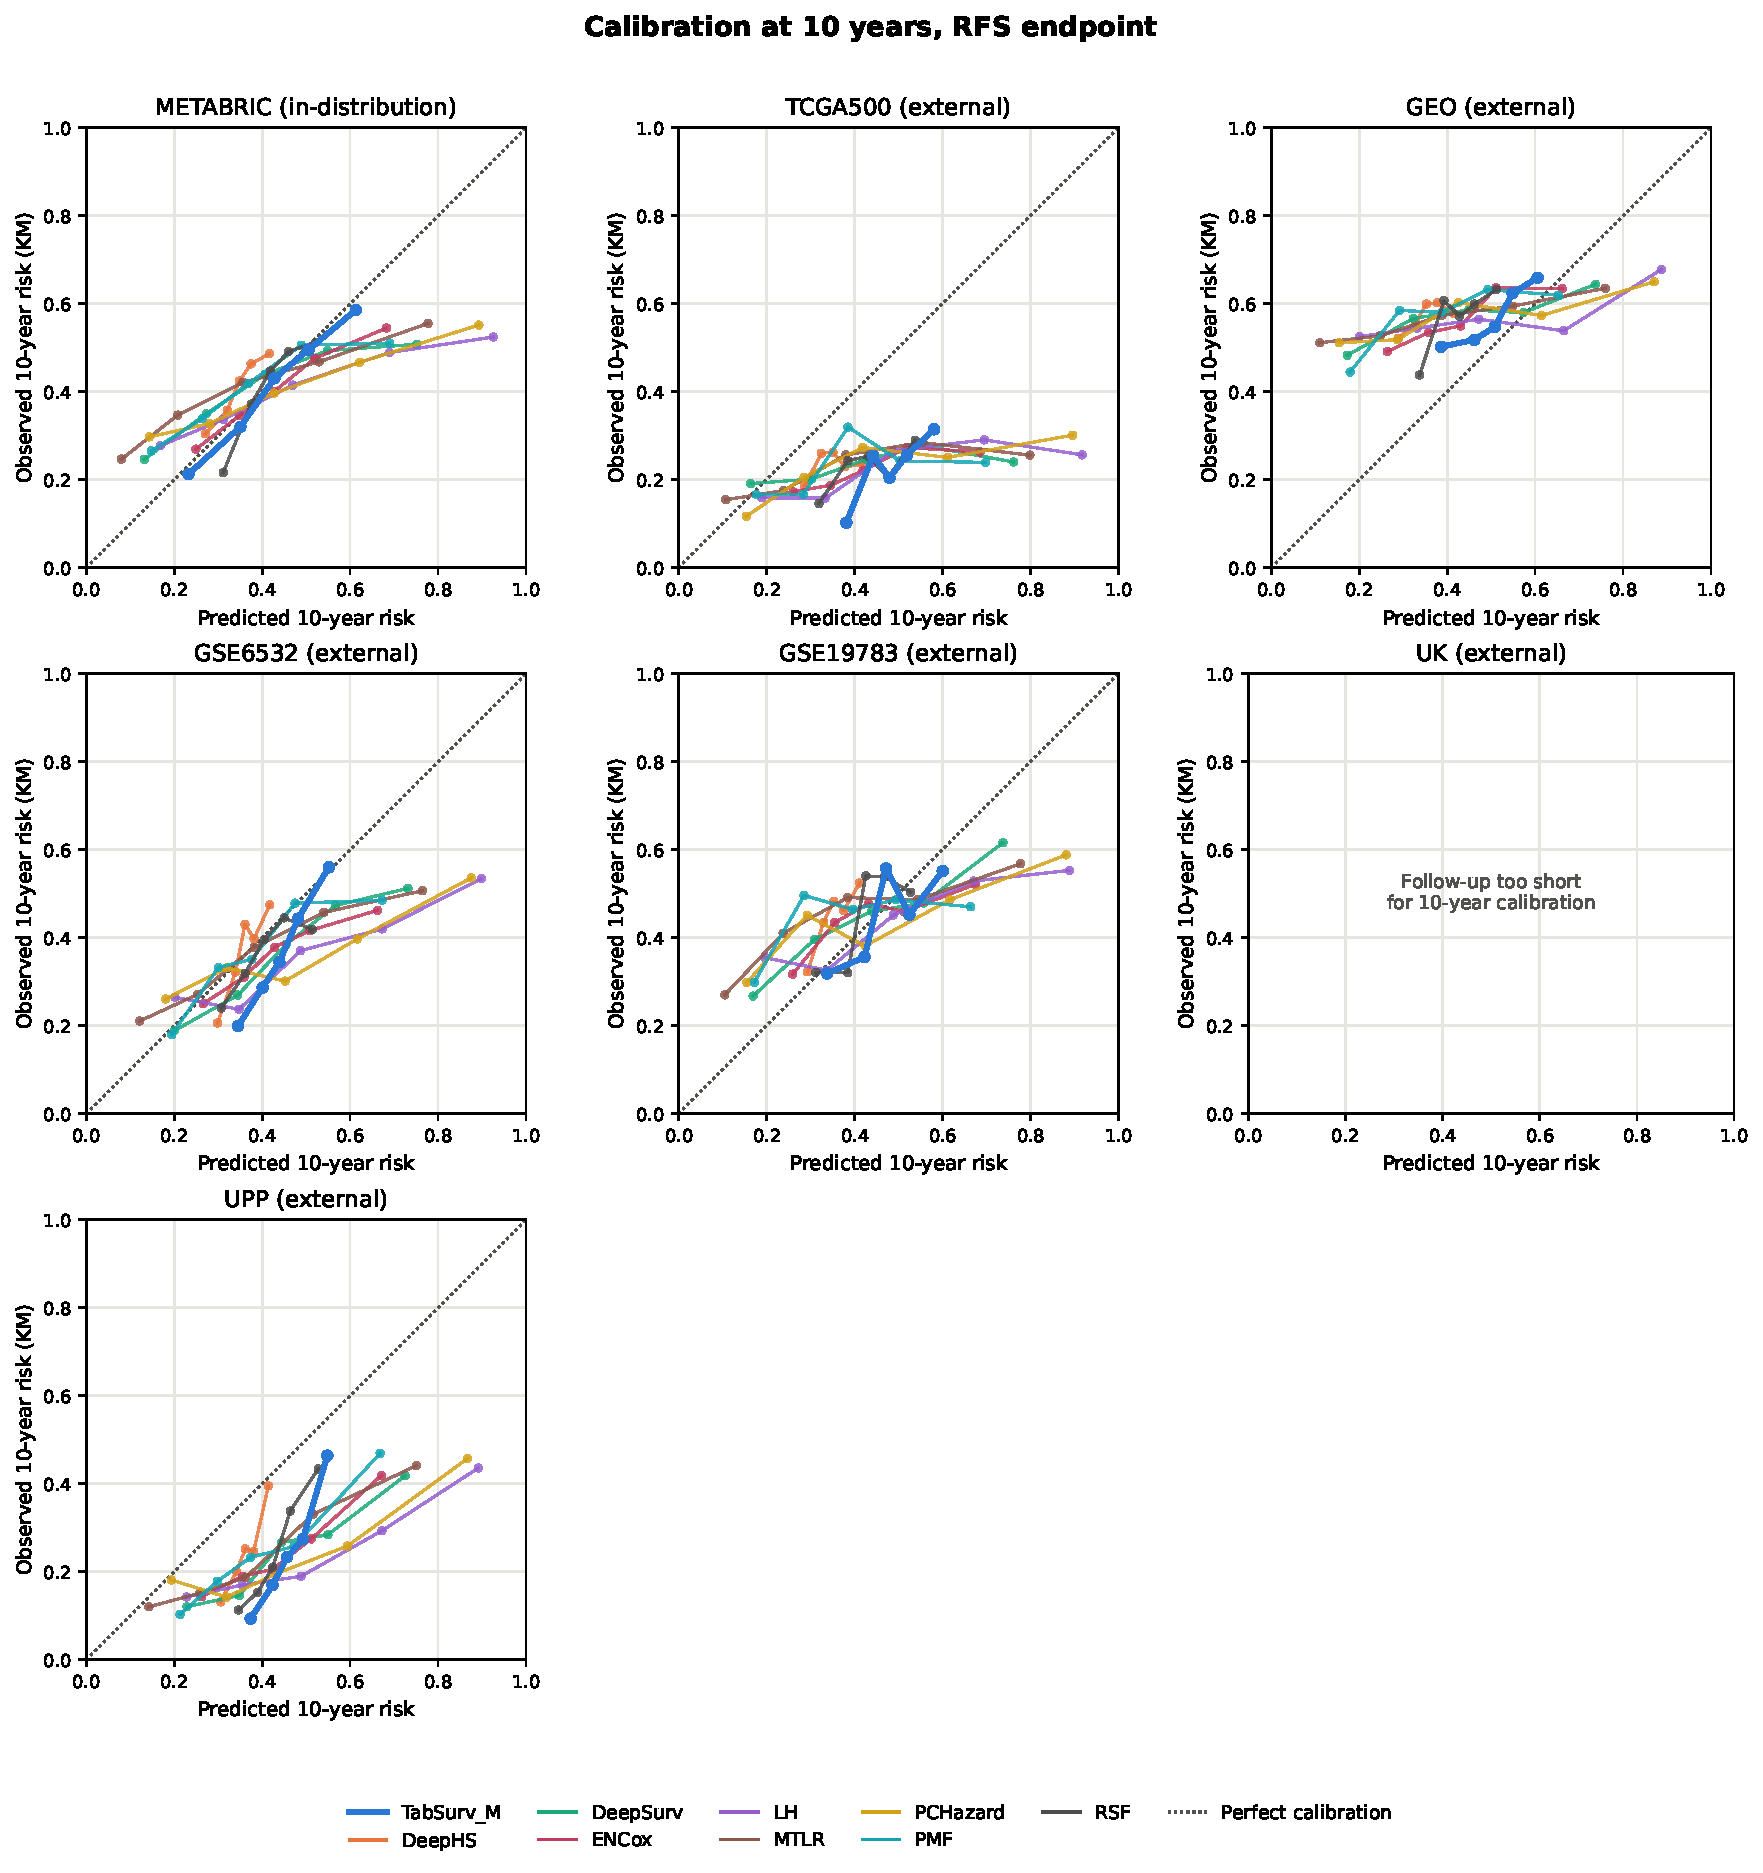
\includegraphics[width=\textwidth]{Fig_S_calibration_RFS_10y.pdf}
\caption{Calibration of predicted 10-year RFS risk in every cohort. Each point is a risk group: mean predicted risk of an event by 10 years against the Kaplan--Meier observed risk in that group, averaged over five seeds. The dotted diagonal marks perfect calibration. TabSurv\_M is shown as a thick blue line. Panels marked as having too short follow-up have no patients at risk beyond 10 years.}
\label{fig:supp_calibration_rfs_10y}
\end{figure*}

\begin{figure*}[t]
\centering
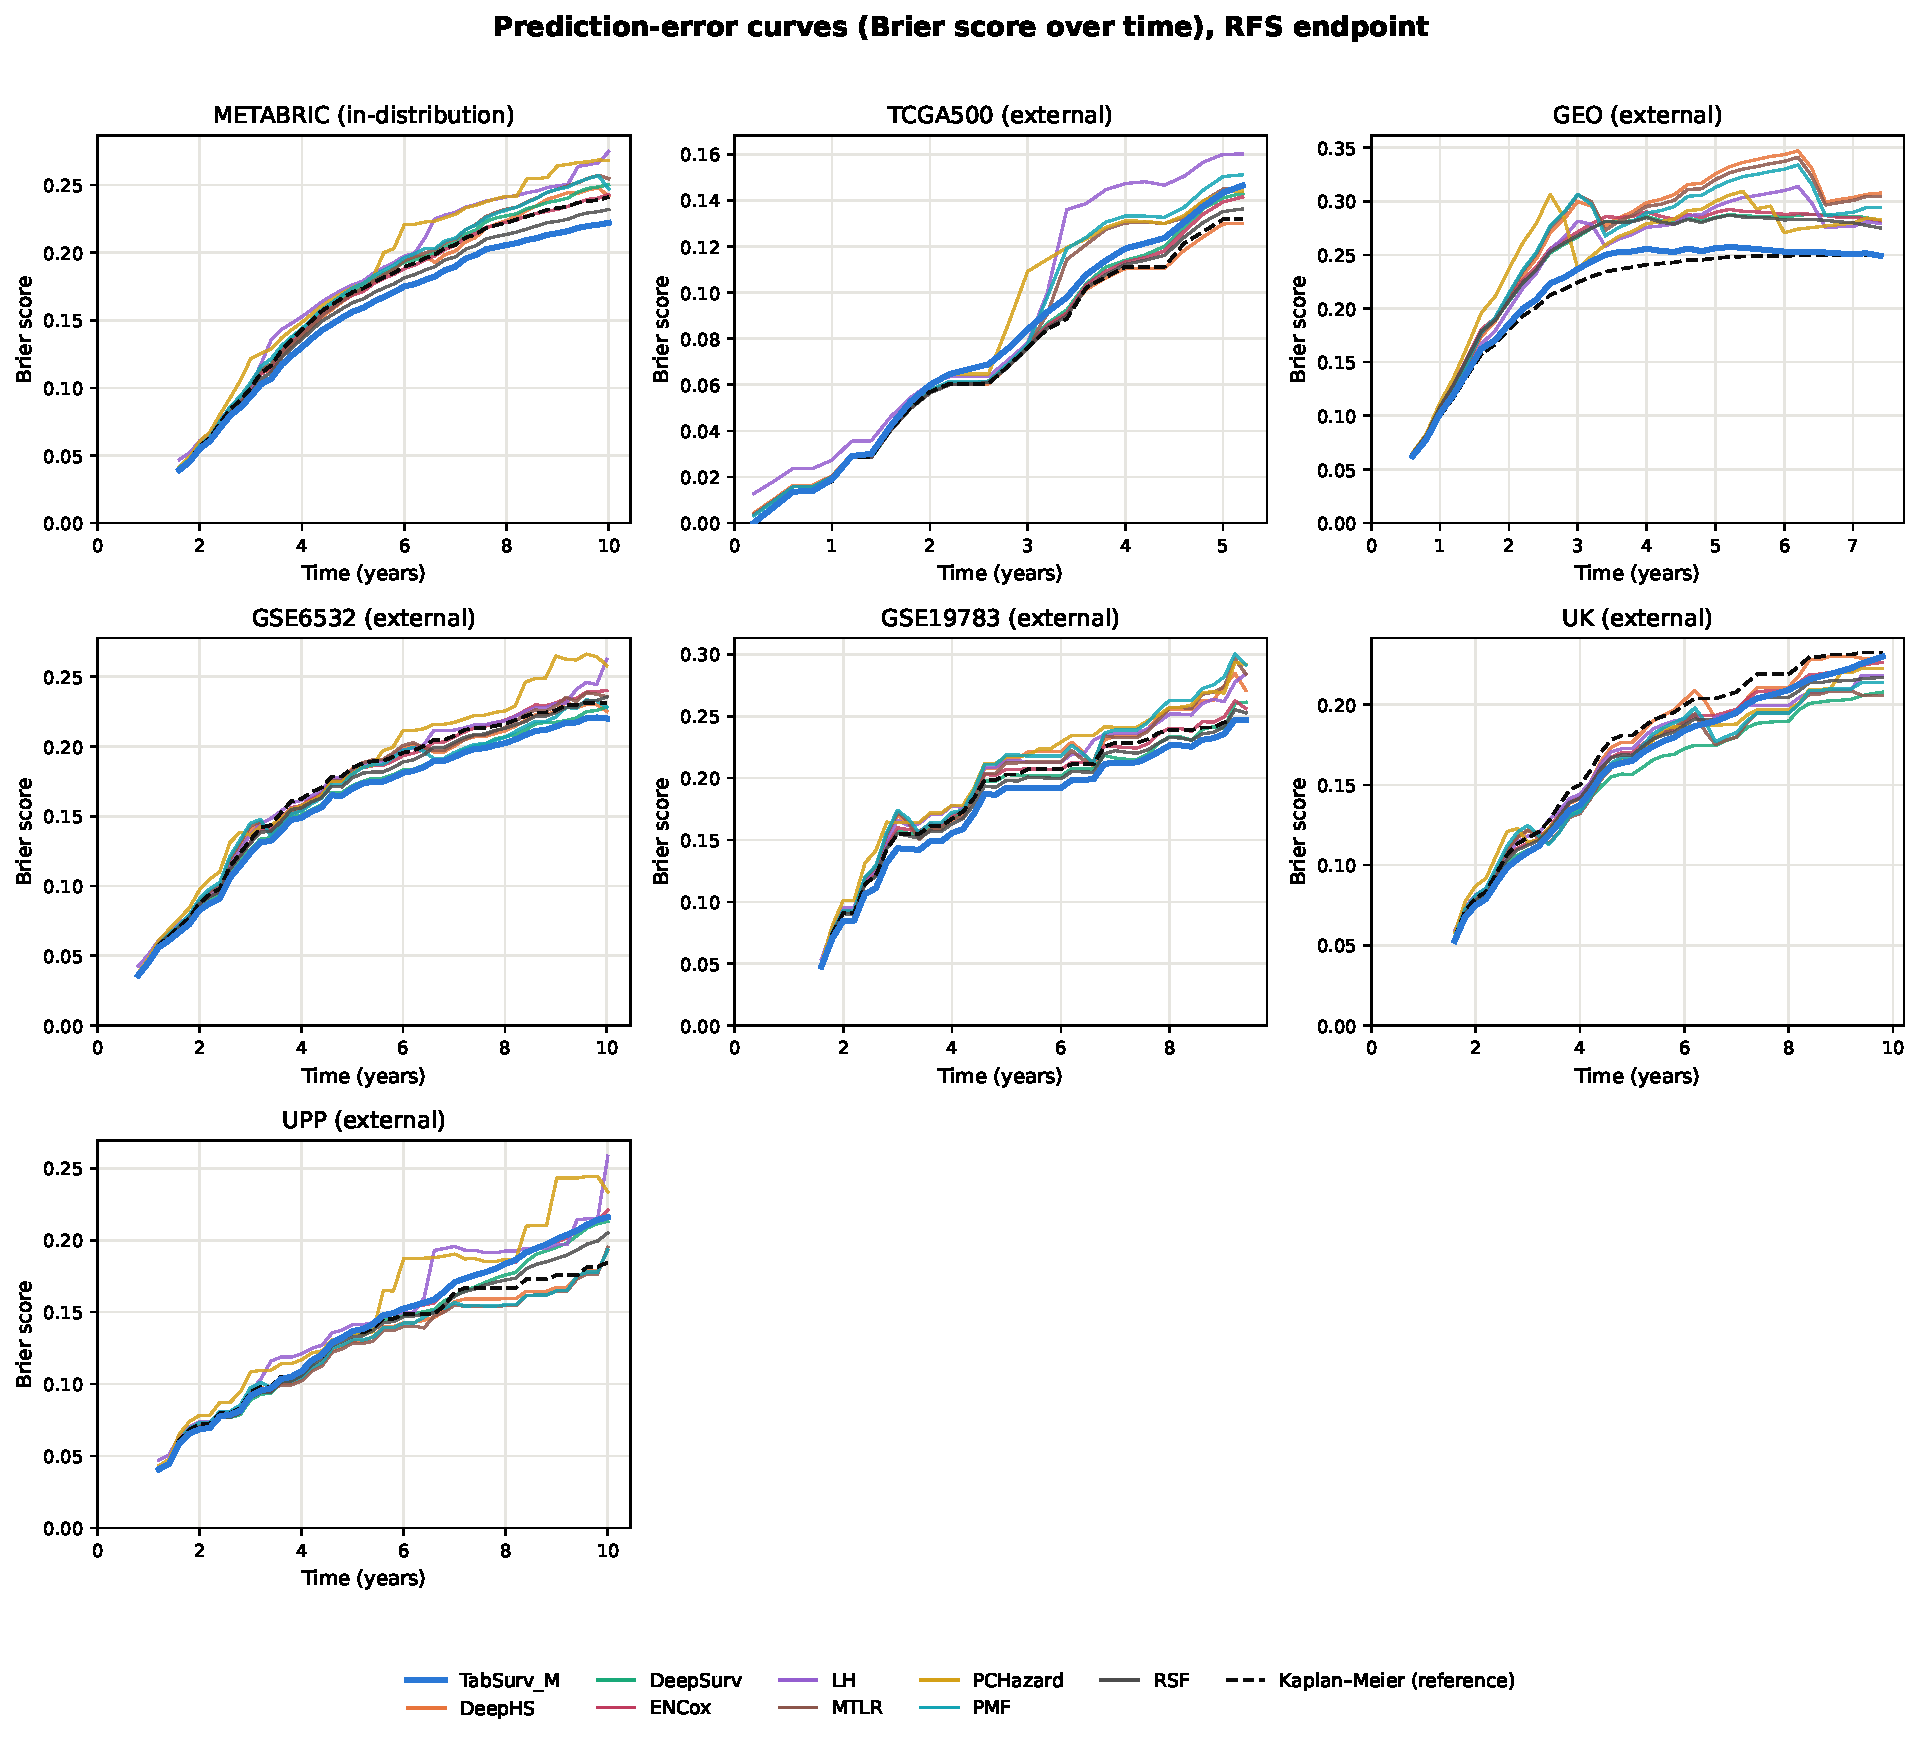
\includegraphics[width=\textwidth]{Fig_S_prediction_error_RFS.pdf}
\caption{Prediction-error curves for the RFS endpoint in every cohort: Brier score over time (lower is better), averaged over five seeds. The dashed black line is the covariate-free Kaplan--Meier reference; a model curve below it indicates that the covariates improve prediction at that time. TabSurv\_M is shown as a thick blue line.}
\label{fig:supp_prediction_error_rfs}
\end{figure*}

\begin{figure*}[t]
\centering
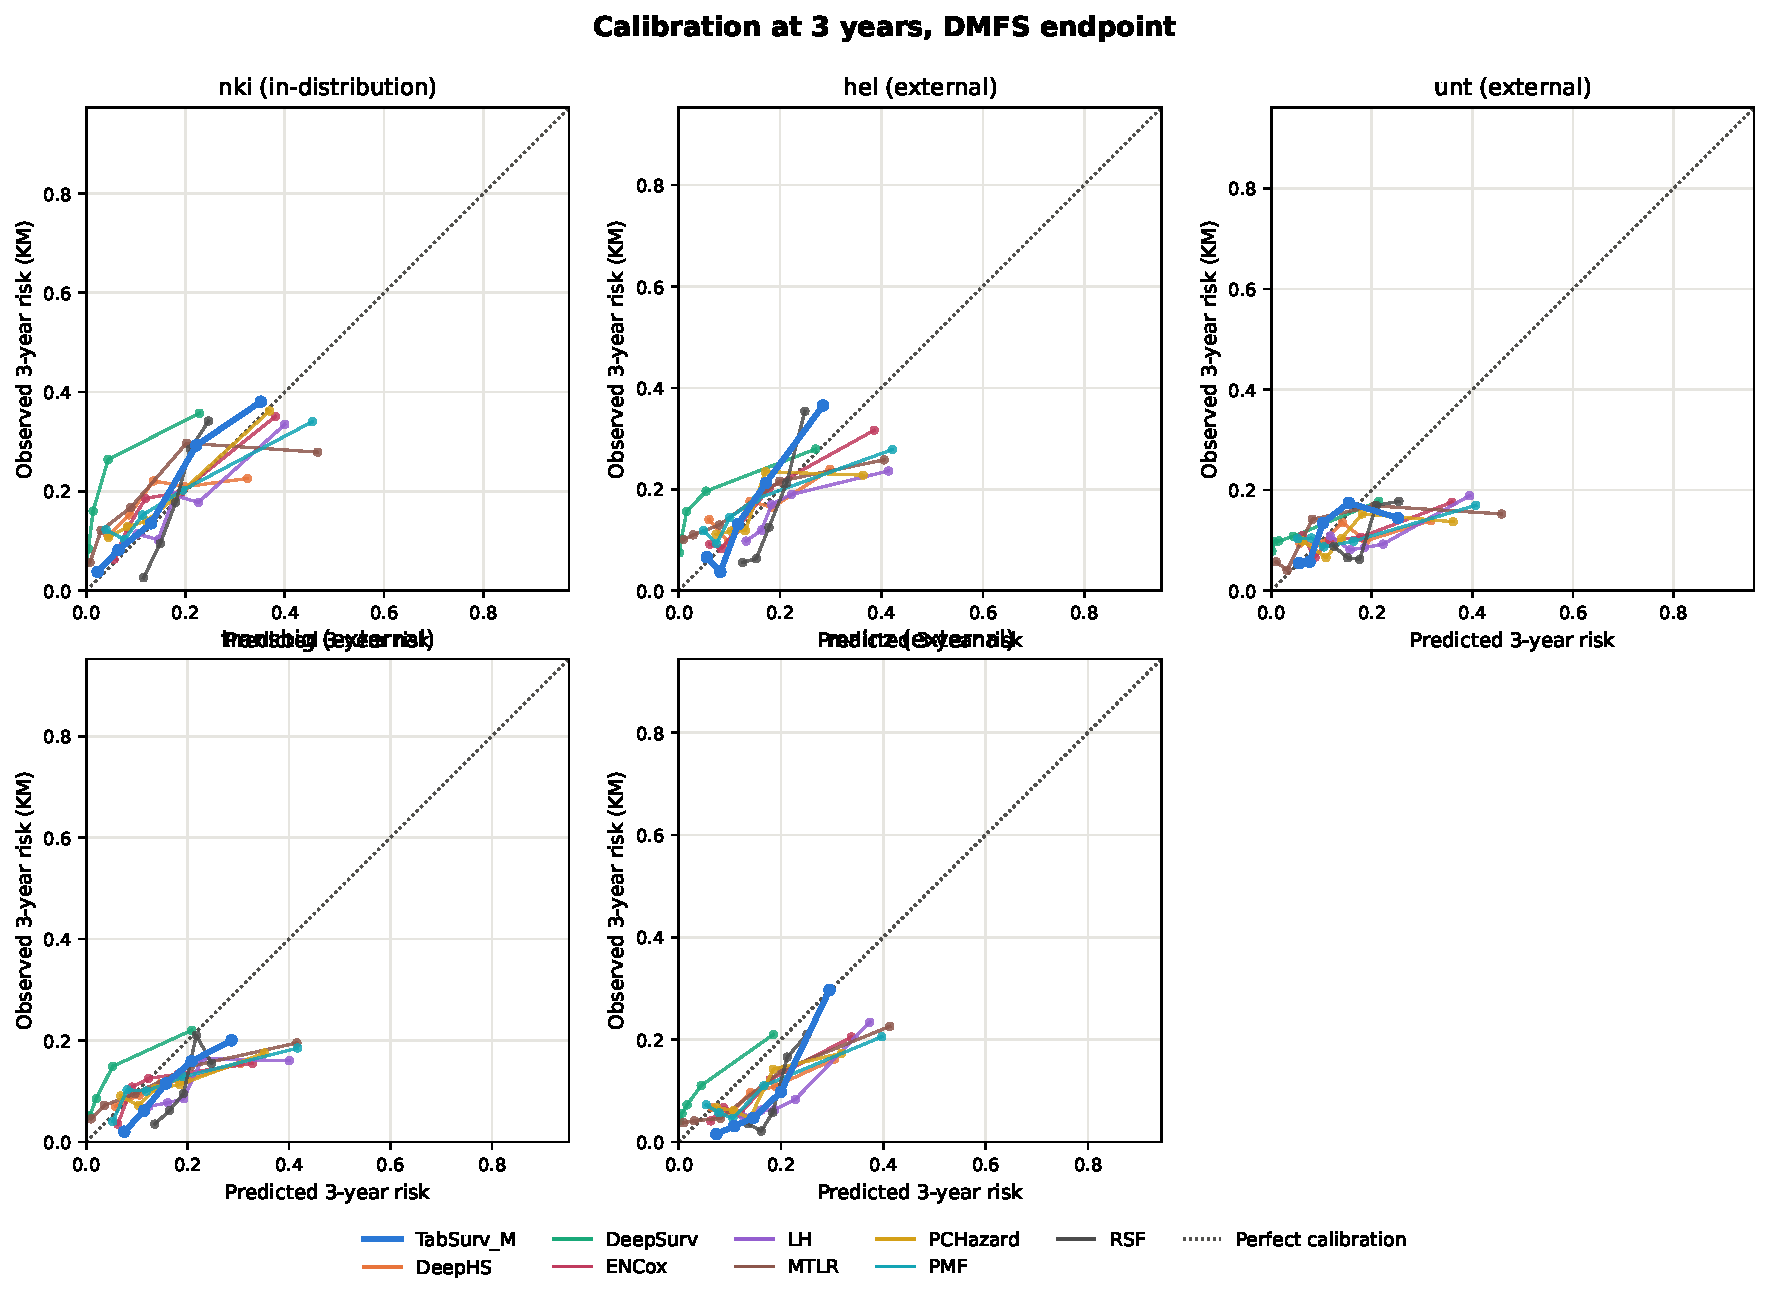
\includegraphics[width=\textwidth]{Fig_S_calibration_DMFS_3y.pdf}
\caption{Calibration of predicted 3-year DMFS risk in every cohort. Each point is a risk group: mean predicted risk of an event by 3 years against the Kaplan--Meier observed risk in that group, averaged over five seeds. The dotted diagonal marks perfect calibration. TabSurv\_M is shown as a thick blue line. Panels marked as having too short follow-up have no patients at risk beyond 3 years.}
\label{fig:supp_calibration_dmfs_3y}
\end{figure*}

\begin{figure*}[t]
\centering
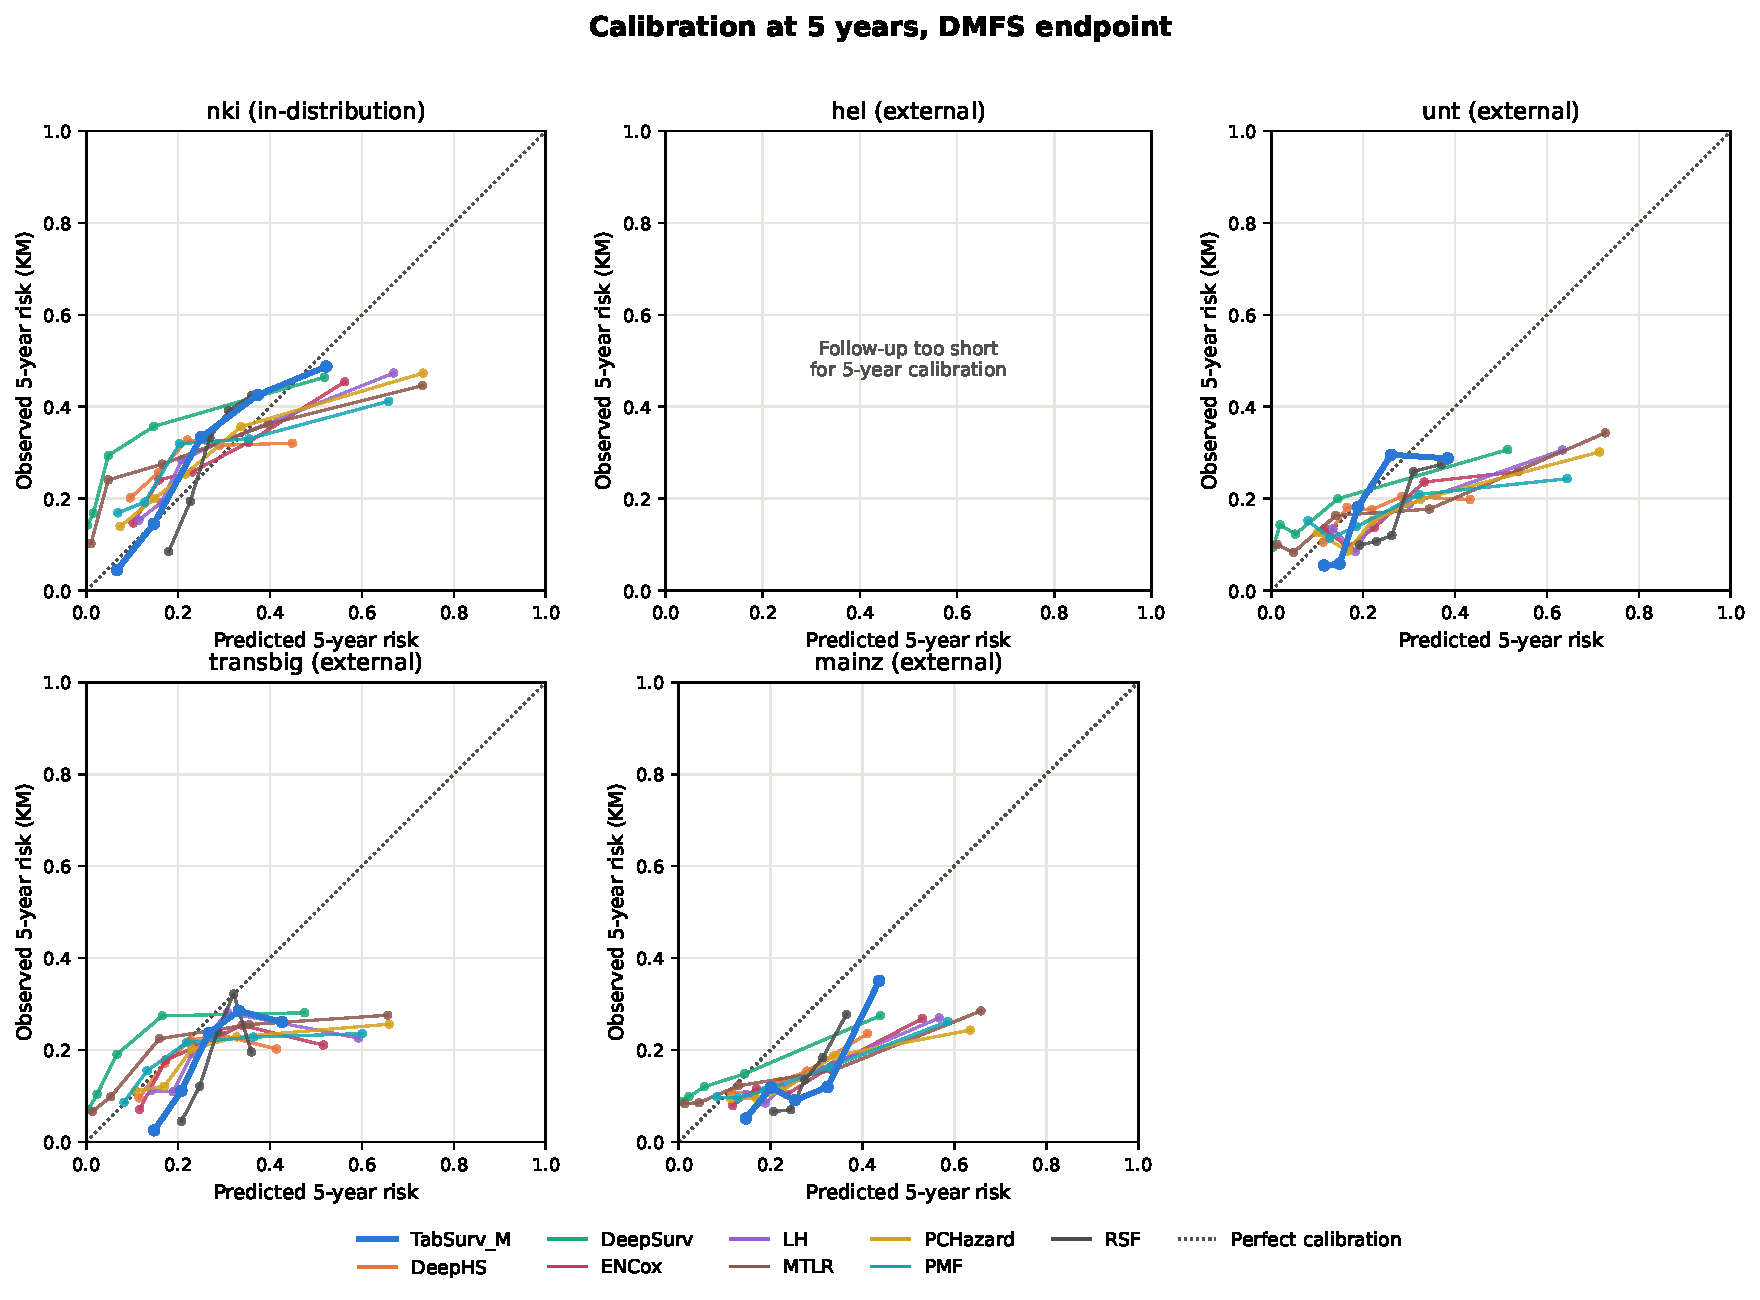
\includegraphics[width=\textwidth]{Fig_S_calibration_DMFS_5y.pdf}
\caption{Calibration of predicted 5-year DMFS risk in every cohort. Each point is a risk group: mean predicted risk of an event by 5 years against the Kaplan--Meier observed risk in that group, averaged over five seeds. The dotted diagonal marks perfect calibration. TabSurv\_M is shown as a thick blue line. Panels marked as having too short follow-up have no patients at risk beyond 5 years.}
\label{fig:supp_calibration_dmfs_5y}
\end{figure*}

\begin{figure*}[t]
\centering
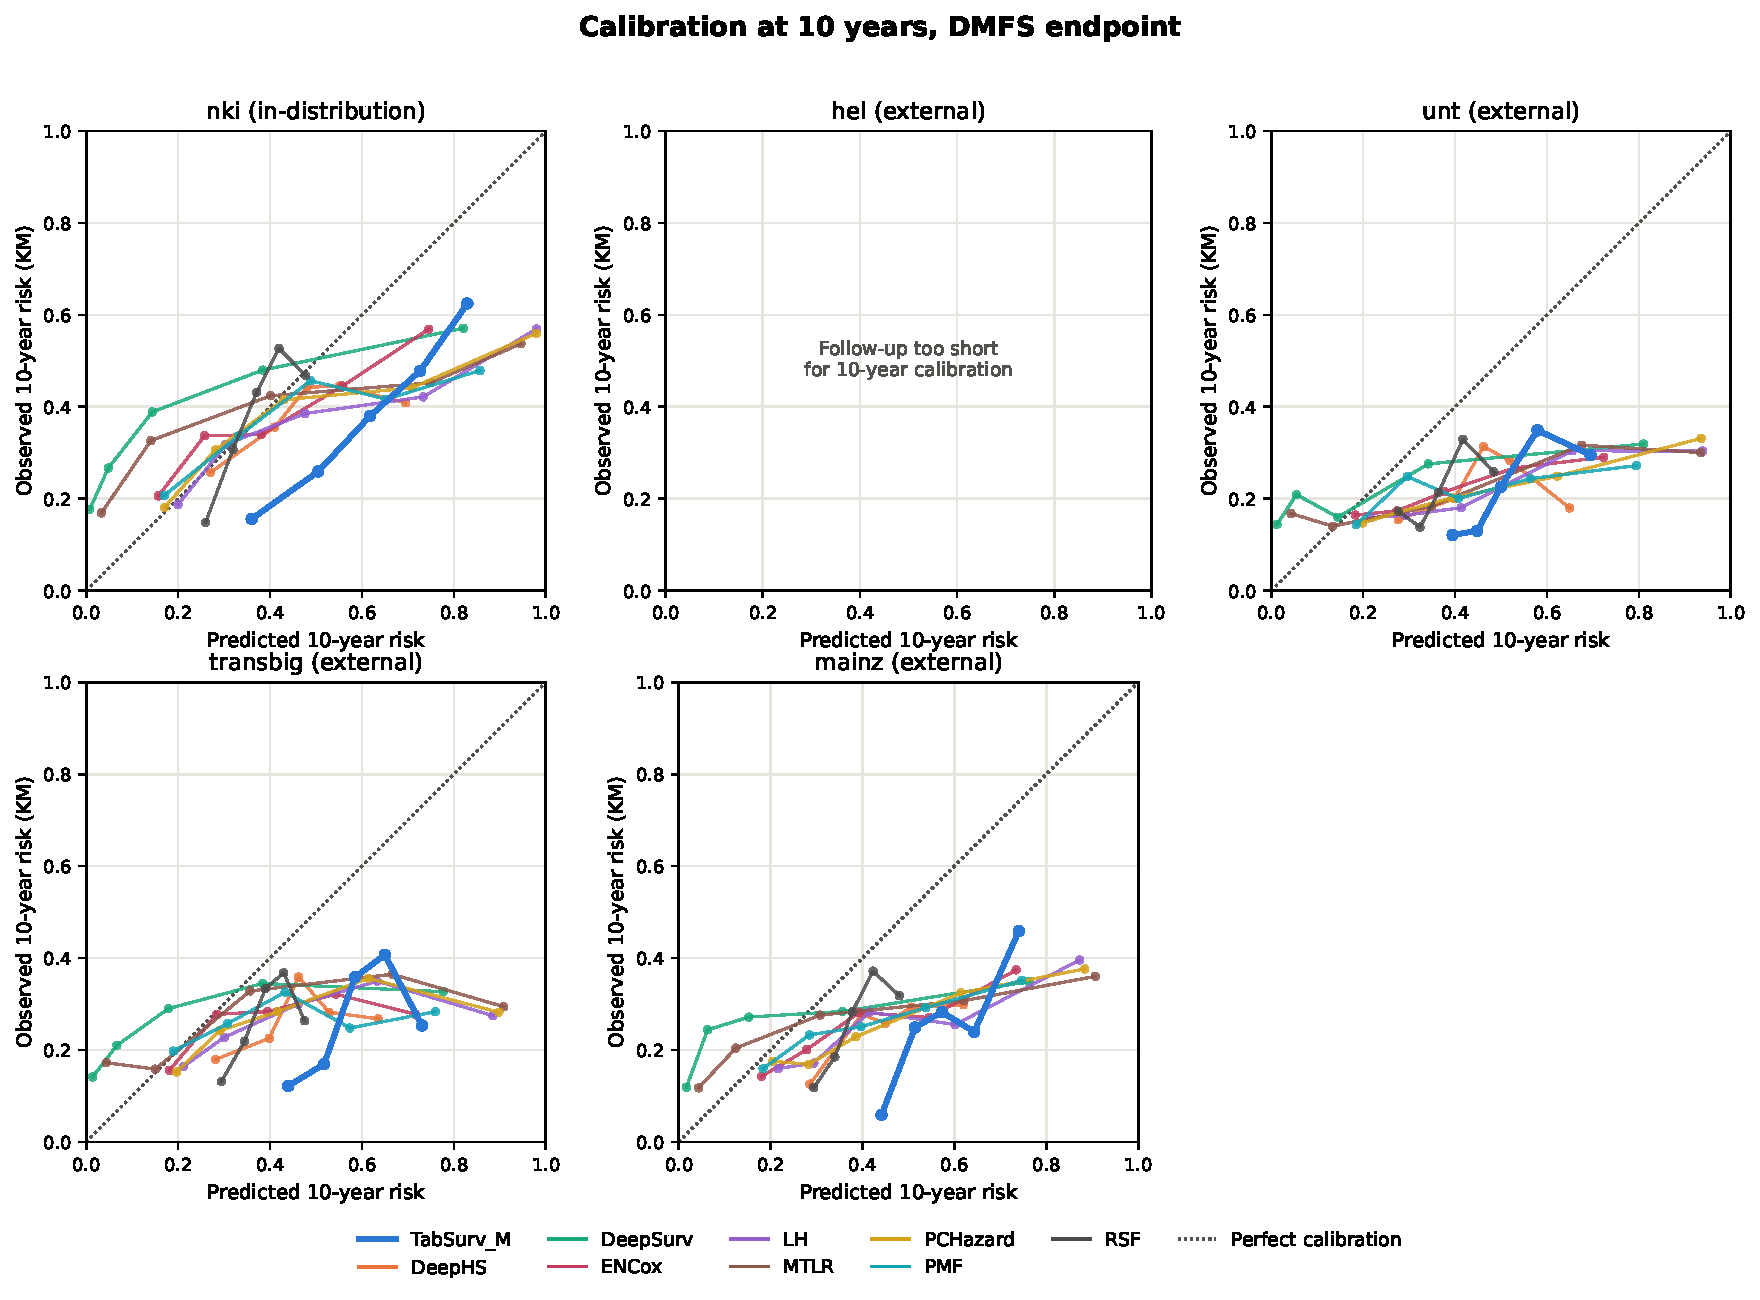
\includegraphics[width=\textwidth]{Fig_S_calibration_DMFS_10y.pdf}
\caption{Calibration of predicted 10-year DMFS risk in every cohort. Each point is a risk group: mean predicted risk of an event by 10 years against the Kaplan--Meier observed risk in that group, averaged over five seeds. The dotted diagonal marks perfect calibration. TabSurv\_M is shown as a thick blue line. Panels marked as having too short follow-up have no patients at risk beyond 10 years.}
\label{fig:supp_calibration_dmfs_10y}
\end{figure*}

\begin{figure*}[t]
\centering
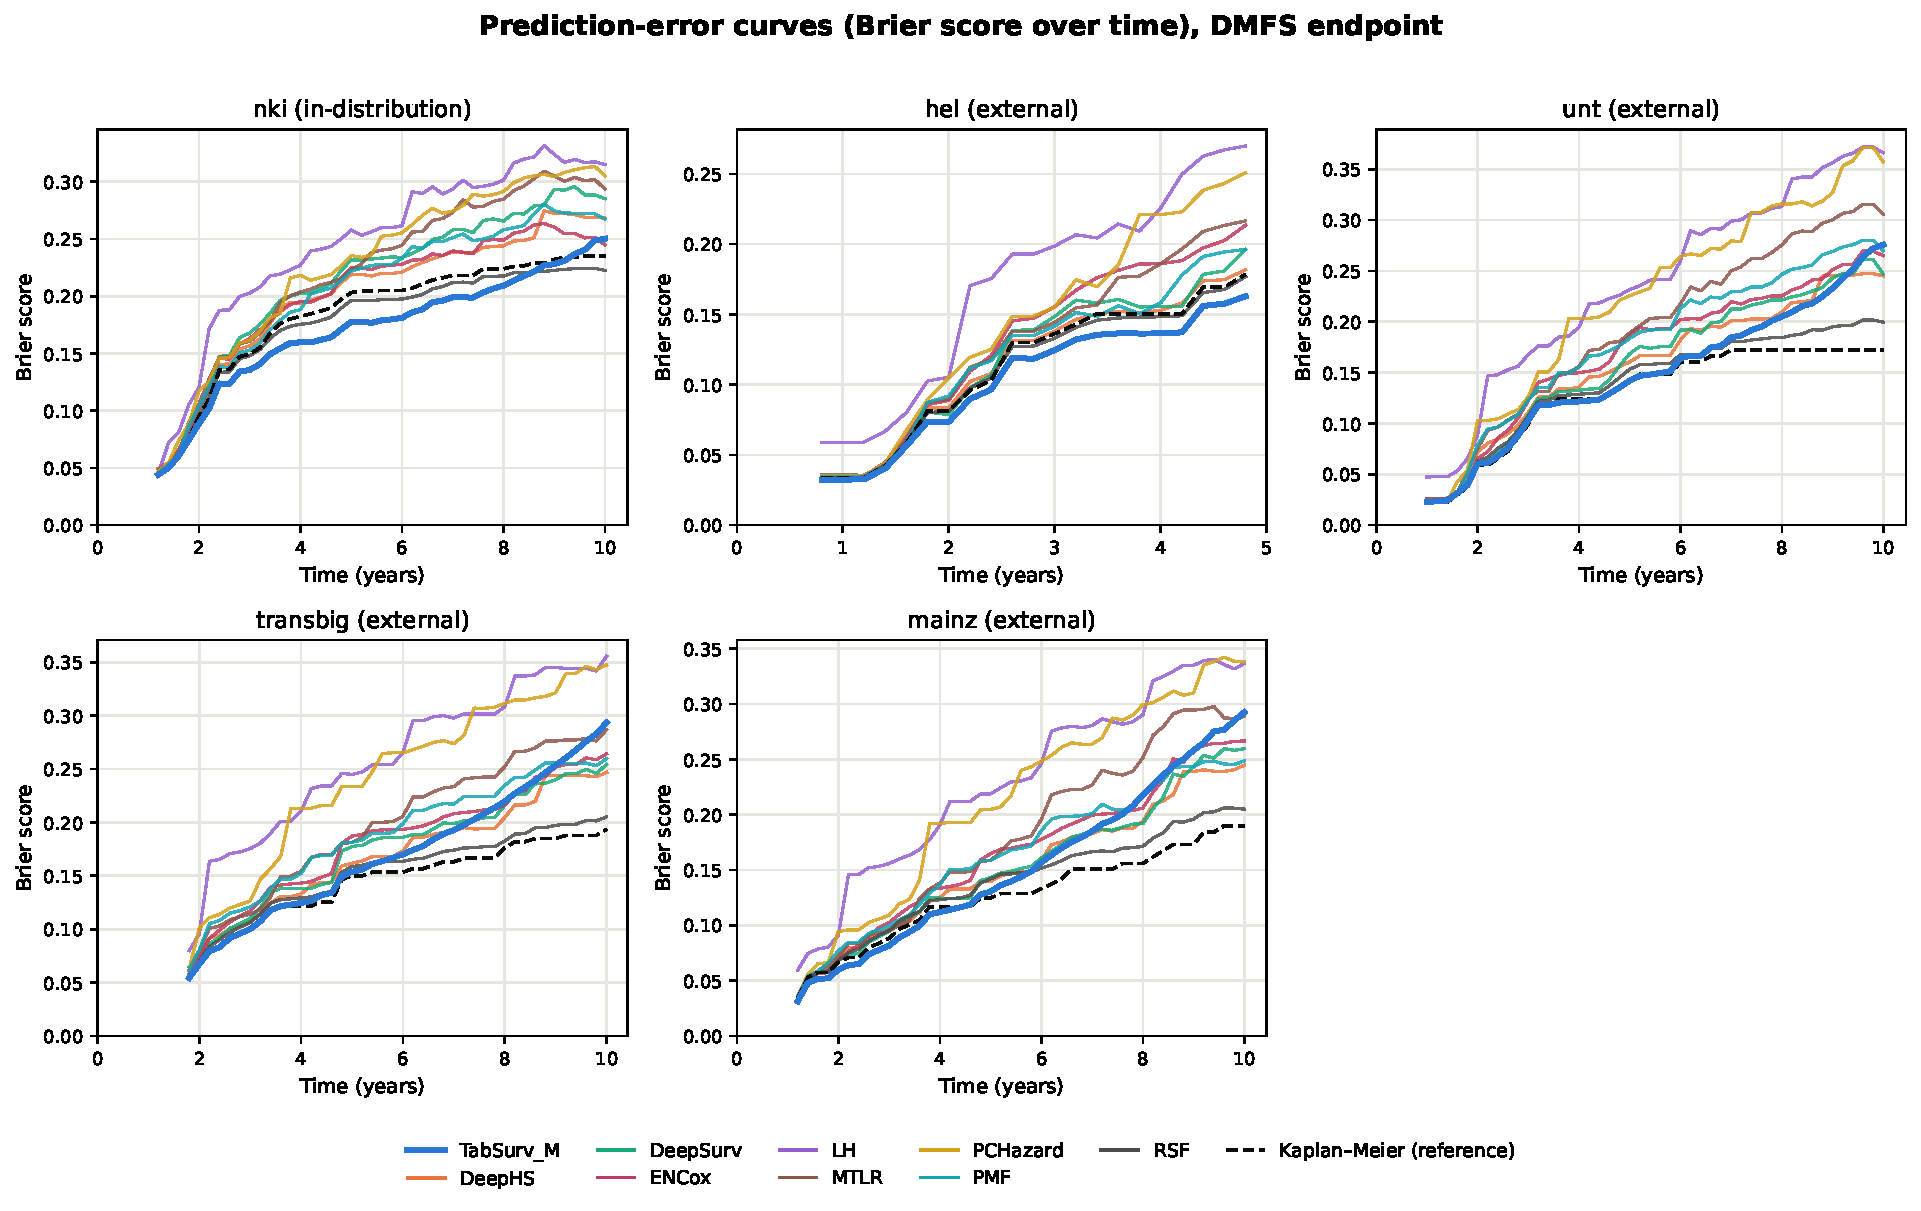
\includegraphics[width=\textwidth]{Fig_S_prediction_error_DMFS.pdf}
\caption{Prediction-error curves for the DMFS endpoint in every cohort: Brier score over time (lower is better), averaged over five seeds. The dashed black line is the covariate-free Kaplan--Meier reference; a model curve below it indicates that the covariates improve prediction at that time. TabSurv\_M is shown as a thick blue line.}
\label{fig:supp_prediction_error_dmfs}
\end{figure*}
